\documentclass[twoside]{article}
\usepackage[a4paper]{geometry}
\geometry{verbose,tmargin=2.5cm,bmargin=2cm,lmargin=2cm,rmargin=2cm}
\usepackage{fancyhdr}
\pagestyle{fancy}

% nastavení pisma a~češtiny
\usepackage{lmodern}
\usepackage[T1]{fontenc}
\usepackage[utf8]{inputenc}
\usepackage[czech]{babel}

% odkazy
\usepackage{url}

\usepackage{float}
% vícesloupcové tabulky
\usepackage{multirow}
\usepackage{amssymb}
\usepackage{gensymb}
\usepackage{bbold}
\usepackage{amsmath}
\usepackage{mathtools}
\usepackage{commath}

% vnořené popisky obrázků
\usepackage{subcaption}

% automatická konverze EPS 
\usepackage{graphicx} 
\usepackage{epstopdf}
\epstopdfsetup{update}

\graphicspath{{./images}}

% odkazy a~záložky
\usepackage[unicode=true, bookmarks=true,bookmarksnumbered=true,
bookmarksopen=false, breaklinks=false,pdfborder={0 0 0},
pdfpagemode=UseNone,backref=false,colorlinks=true] {hyperref}

% Poznámky při překladu
\usepackage{xkeyval}	% Inline todonotes
\usepackage[textsize = footnotesize]{todonotes}
\presetkeys{todonotes}{inline}{}

%https://tex.stackexchange.com/questions/2783/bold-calligraphic-typeface
\DeclareMathAlphabet\mathbfcal{OMS}{cmsy}{b}{n}

% Zacni sekci slovem ukol
\renewcommand{\thesection}{Úkol \arabic{section}}
% enumerate zacina s pismenem
\renewcommand{\theenumi}{\alph{enumi}}

% smaz aktualni page layout
\fancyhf{}
% zahlavi
\usepackage{titling}
\fancyhf[HC]{\thetitle}
\fancyhf[HLE,HRO]{\theauthor}
\fancyhf[HRE,HLO]{\today}
 %zapati
\fancyhf[FLE,FRO]{\thepage}

% údaje o autorovi
\title{Automatické řízení: DÚ 9 -- Polynomiální metody}
\author{Vojtěch Michal}
\date{\today}

\begin{document}

\maketitle

Jsem narozen 18. února 2000. Proto volím $d = 1$, $r = 2$, $m = 2$.

\section{Diofantická rovnice}

Řešte polynomiální rovnici
\begin{equation}
	\label{eq:zadani}
	\underbrace{(2 + 3s + s^2)}_{=a(s)}x(s) + \underbrace{(1 + s)}_{=b(s)}y(s) = \underbrace{5 + 8s + 4s^2 + s^3}_{=c(s)}
\end{equation}
\begin{itemize}
	\item Rovnici řešte elementárními operacemi na polynomiální matici. Najděte obecné řešení.
	\item Rovnici řešte pomocí Sylvestrovy matice. Najděte obecné řešení.
	\item Najděte řešení minimálního stupně v x.
	\item Najděte řešení minimálního stupně v y.
	\item Nakonec řešte přímo funkcí \textit{axbyc} Polynomial Toolboxu, a to pro všechny typy řešení
	minimálních stupňů.
\end{itemize}

\textbf{Řešení:}
Jsou dány polynomy
\begin{equation}
	\begin{aligned}
		a(s) &= s^2 + 3s + 2 = (s+1)(s+2), \\
		b(s) &= s + 1, \\
		c(s) &= s^3 + 4s^2 + 8s + 5 = (s+1)(s^2 + 3s + 5).
	\end{aligned}
\end{equation} \\
Bude se mi hodit znát hodnotu
\begin{equation}
	g(s) = \text{gcd}(a(s), b(s)) = s + 1
\end{equation}
a od něj odvozených
\begin{equation}
	\label{eq:bar_poly}
	\begin{aligned}
		\bar{a}(s) &= \frac{a(s)}{g(s)} = s + 2, \\
		\bar{b}(s) &= \frac{b(s)}{g(s)} = 1. \\
	\end{aligned}
\end{equation}

Diofantická rovnice v polynomech bude mít řešení právě tehdy, když $\text{gcd}(a(s), b(s))$ dělí beze zbytku $c(s)$. Protože polynom $c(s)$ má kořen -1,
je beze zbytku dělitelný polynomem $g(s)$ a řešení Diofantické rovnice tedy má smysl hledat.
Rovnici \eqref{eq:zadani} lze vykrácením společného dělitele obou stran $g(s)$ zjednodušit na
\begin{equation}
	\label{eq:easy}
	\underbrace{(s+2)}_{\bar{a}(s)} x(s) + \underbrace{1}_{\bar{b}(s)} y(s) = \underbrace{s^2 + 3s +5}_{\bar{c}(s)},
\end{equation}
kterou budeme následně řešit různými postupy.

\subsection{Polynomiální maticové redukce}
Ze zadaných polynomů $a(s)$, $b(s)$ utvořím matici
\begin{equation}
	\mathbf{M} = \begin{bmatrix}
		a(s) & 1 & 0 \\
		b(s) & 0 & 1 \\
	\end{bmatrix} = \begin{bmatrix}
		s^2 + 3s + 2 & 1 & 0 \\
		s+1 & 0 & 1
	\end{bmatrix},
\end{equation}
kterou následně upravím elementárními operacemi. Nejprve odečtu od prvního řádku $(s+2)$ krát druhý řádek
\begin{equation}
	\begin{bmatrix}
		0 & 1 & -s-2 \\
		s+1 & 0 & 1
	\end{bmatrix},
\end{equation}
řádky první a druhý prohodím a použiji standardní označení
\begin{equation}
	\begin{bmatrix}
		s+1 & 0 & 1 \\
		0 & 1 & -s-2 
	\end{bmatrix} = \begin{bmatrix}
		g(s) & p(s) & q(s) \\
		0 & v(s) & w(s)
	\end{bmatrix}.
\end{equation}

První kontrola správnosti je ověření, že v levém horním rohu je skutečně $\text{gcd}(a(s), b(s))$.
Dále by dle Bezoutovy věty mělo platit
\begin{equation}
	\begin{aligned}
		p(s)a(s) + q(s)b(s) &= g(s) \\
		v(s)a(s) + w(s)b(s) &= 0, \\
	\end{aligned}
\end{equation}
což je zřejmě splněno. Rozložme $c(s) = g(s)\bar{c}(s) \Rightarrow \bar{c}(s) = s^2 + 3s + 5$.
Partikulární řešení zadané diofantické rovnice je 
\begin{equation}
	\label{eq:partikularni}
	\begin{aligned}
		x_p(s) &= p(s) \bar{c}(s) = 0, \\
		y_p(s) &= q(s) \bar{c}(s) = s^2 + 3s + 5.
	\end{aligned}
\end{equation}

Dosazením polynomů \eqref{eq:partikularni} do \eqref{eq:zadani} vyjde identita
\begin{equation}
	(2 + 3s + s^2)0 + (1 + s)(s^2 + 3s + 5) = (s+1)(s^2 + 3s + 5),
\end{equation}
která je jistě splněna a polynomy $x_p(s)$ a $y_p(s)$ jsou skutečně partikulární řešení zadané diofantické rovnice.

\subsection{Sylvestrova matice}
Pro řešení polynomiální Diofantické rovnice je potřeba odhadnout stupeň polynomů $x(s)$, $y(s)$
a následně sestavit Sylvestrovu matici $\mathbf{S}$. Aby byla Sylvestrova matice regulární, musí být polynomy nesoudělné,
proto vyjdu z rovnice \eqref{eq:easy}. Pro polynomy $\bar{a}(s) = s+2$ a $\bar{b}(s) = 1$ je Sylvestrova matice
\begin{equation}
	\mathbf{S} = \begin{bmatrix}
		\bar{a}_0 & \bar{a}_1 & 0 \\
		\bar{b}_0 & \bar{b}_1 & 0 \\
		0 & \bar{a}_0 & \bar{a}_1 \\
		0 & \bar{b}_0 & \bar{b}_1 
	\end{bmatrix} = \begin{bmatrix}
			2 &   1 &        0\\
			1 &        0 &        0\\
		   0  &  2  &  1               \\
		   0  &  1  &       0
	\end{bmatrix}.
\end{equation}

Protože $\text{deg }\bar{c}(s)$ = 2 a max(deg $\bar{a}(s)$, deg $\bar{b}(s)$) = 1, 
odhaduji, že polynomy v řešení budou mít stupeň 1. Proto $x(s) = x_1 s + x_0$,  $y(s) = y_1 s + y_0$.
Odtud se problém řešení Diofantické rovnice převádí na řešení soustavy
\begin{equation}
	\underbrace{
	\begin{bmatrix}
		x_0 & y_0 & x_1 & y_1
	\end{bmatrix}}_{X^T}
	\mathbf{S} = \underbrace{\begin{bmatrix}
		c_0 & c_1 & c_2 
	\end{bmatrix}}_{C^T} = \begin{bmatrix}
		5 & 3 & 1
	\end{bmatrix}.
\end{equation}
Tuto maticovou rovnici transponuji
\begin{equation}
	X^T \mathbf{S} = C^T \Rightarrow \mathbf{S}^T X = C,
\end{equation}
rozepsáno po prvcích
\begin{equation}
	\begin{bmatrix}
		2   & 1  &       0    &     0\\
		1   &      0  &  2    &1\\
			 0   &      0  &   1    &     0
	\end{bmatrix} \begin{bmatrix}
		x_0 \\ y_0 \\ x_1 \\ y_1
	\end{bmatrix} = \begin{bmatrix}
		5 \\ 3 \\ 1 
	\end{bmatrix},
\end{equation}
což je standardní soustava lineárních rovnic, kterou lze řešit pomocí Gauss-Jordanovy eliminace
na rozšířenou matici soustavy
	\begin{equation}
\left[
\begin{array}{cccc|c}
	2 & 1 & 0 & 0 & 5\\
	1 & 0 & 2 & 1 & 3\\
	0 & 0 & 1 & 0 & 1
\end{array}
\right].
\end{equation}

Druhý řádek vynásobím mínus dvěma, přičtu první řádek a čtyřikrát třetí:
\begin{equation}
	\left[
\begin{array}{cccc|c}
	2 & 1 & 0 & 0 & 5\\
	1 & 0 & 2 & 1 & 3\\
	0 & 0 & 1 & 0 & 1
\end{array}
\right] \approx
	\left[
		\begin{array}{cccc|c}
			2 & 1 & 0 & 0 & 5\\
			-2 & 0 & -4 & -2 & -6\\
			0 & 0 & 1 & 0 & 1
		\end{array}
		\right] \approx 	\left[
			\begin{array}{cccc|c}
				2 & 1 & 0 & 0 & 5\\
				0 & 1 & 0 & -2 & 3\\
				0 & 0 & 1 & 0 & 1
			\end{array}
			\right].
	\end{equation}

Upravená soustava rovnic je 
\begin{equation}
	\label{eq:soustava}
	\begin{aligned}
		2x_0 + y_0 &= 5,\\
		y_0 - 2 y_1 &= 3, \\
		x_1 &= 1.
	\end{aligned}
\end{equation}
Protože je podurčená, volím $y_1 = K \in \mathbb{R}$ a dosadím do \eqref{eq:soustava}. Hledané koeficienty polynomů proto jsou
\begin{equation}
	\begin{aligned}
		2x_0 + y_0 &= 5 \Rightarrow x_0 = \frac{5-3 - 2 K}{2} = 1-K,\\
		y_0 - 2 K &= 3 \Rightarrow y_0 = 3 + 2K, \\
		x_1 &= 1.
	\end{aligned}
\end{equation}
a parametrizované partikulární řešení diofantické rovnice je
\begin{equation}
	\begin{aligned}
		x(s) &= (1-K) + s, \\
		y(s) &= (3+2K) + Ks,
	\end{aligned}
	\label{eq:obecne_param}
\end{equation}
pro libovolnou reálnou hodnotu $K$. Například volbou $K = 0$ vyjde řešení minimální v y (viz \eqref{eq:minimalni_y}).
Zkoušku provedu dosazením z \eqref{eq:obecne_param} do \eqref{eq:easy}:
\begin{equation}
	\begin{aligned}
		(s+2)(s + (1-K)) + Ks + (3+2K) &= s^2 + 3s + 5\\
		s^2 + s - Ks + 2s + 2-2K + Ks + 3 + 2K &= s^2 + 3s + 5 \\
		s^2 + s(K-K) + 3s  + 2 (K-K) + 5 &= s^2 + 3s + 5
	\end{aligned}
\end{equation}
a tato identita jistě platí.

\subsection{Řešení minimální v x}
\textit{Řešení minimální v x} je takové, pro které platí deg $x(s)$ < deg $\bar{b}(s)$. Protože je však $\bar{b}(s)$
polynom stupně nula (je to nenulová konstanta), lze rovnou určit $x(s) = 0$, protože neexistuje jiný polynom se stupněm nižším než nula.
Protože jsou minimální řešení unikátní, odpovídá toto řešení partikulárnímu řešení nalezenému v rovnici \eqref{eq:partikularni}.

\subsection{Řešení minimální v y}
\textit{Řešení minimální v y} je takové, pro které platí deg $y(s)$ < deg $\bar{a}(s)$. Protože deg $\bar{a}(s) = 1$,
hledám polynom $y(s)$ jako nenulovou konstantu. Hledám polynomy $p(s)$, $r(s)$ tak, aby platilo $y_p(s) = \bar{a}(s)p(s) + r(s)$.
Po Euklidově dělení pro výpočet $y_p(s)/\bar{a}(s)$ vychází
\begin{equation}
	\begin{aligned}
		p(s) &= s+1, \\
		r(s) &= 3.
	\end{aligned}
\end{equation}
Obecné řešení rovnice \eqref{eq:easy} má po dosazení z rovnic \eqref{eq:bar_poly} a \eqref{eq:partikularni} tvar
\begin{equation}
	\begin{aligned}
		x &= x_p(s) - \bar{b}(s) \cdot t(s) = - t(s), \\
		y &= y_p(s) + \bar{a}(s) \cdot t(s) = (s^2 + 3s + 5) + (s+2)t(s),
	\end{aligned}
	\label{eq:obecne_reseni}
\end{equation}
kde $t(s)$ je libovolný polynomiální parametr. Postavím $t(s) = -p(s)$, poté řešení minimální v y je
\begin{equation}
	\begin{aligned}
		x(s) &= 0 - 1 (-s-1) &= s+1, \\
		y(s) &= (s^2 + 3s +5) - (s+2) \cdot (s+1) &= 3.
	\end{aligned}
	\label{eq:minimalni_y}
\end{equation}

\subsection{Řešení funkcí \textit{axbyc}}
Volání Matlabovské funkce \textit{axbyc} s polynomy $a(s)$, $b(s)$, $c(s)$ vrací následující výsledky:
\begin{itemize}
	\item Pro \textit{axbyc}(a, b, c,\textbf{'minx'}) jsou nalezené polynomy $x(s) = 0$, $y(s) = s^2 + 3s + 5$.
	\item Pro \textit{axbyc}(a, b, c,\textbf{'miny'}) jsou nalezené polynomy $x(s) = s+1$, $y(s) = 3$.
\end{itemize}

\section{Asymptotické sledování}
Pro soustavu s přenosem
\begin{equation}
	\label{eq:prenos}
	G(s) = \frac{b(s)}{a(s)} = \frac{s+2}{s(s-1)}
\end{equation}

\begin{itemize}
	\item  Navrhněte polynomiálními metodami regulátor se dvěma stupni volnosti, který zajistí asymptotické
	sledování ramp. Póly výsledného systému umístěte do poloh $s_{1,2} = -2 \pm j$. Bude-li potřeba 3. pól, vykraťte
	jím nulu soustavy.
 	\item Vypočtěte přenos výsledného systému z reference na výstup soustavy. Překontrolujte, zda odpovídá
	požadavkům.
	\item Vykreslete odezvu výsledného systému na skok reference a na rampu reference
\end{itemize}

\textbf{Řešení:} 
Regulátor se dvěma stupni volnosti představuje polynomy $r(s)$, $p(s)$, $q(s)$ (pro schéma viz slide 12 \cite{sebek}).

V systému jsou přenos z reference na výstup systému
\begin{equation}
	y(s) = \underbrace{\frac{br}{ap+bq}}_{=G(s)}  y_r(s).
\end{equation}

Řád výsledného systému vyberu pomocí požadavku na ryzost regulátoru. Aby byl ryzí regulátor,
musí být deg $c(s) \ge$ 2deg $a(s)$, kde $c(s)$ je char. polynom uzavřené ZV. 
Protože deg $a(s)$ = 2, vyžaduje toho kritérium, aby celkový systém byl řádu tři a měl charakteristický polynom
\begin{equation}
	c(s) = (s + 2 + j)(s + 2 - j)(s+2),
\end{equation}
kde první dva póly jsou dány požadavky zadavatele, třetím pólem vykracujeme stabilní nulu.

Pro nalezení regulátoru řeším Diofantickou rovnici
\begin{equation}
	a(s)p(s) + b(s)q(s) = c(s)
\end{equation}
se zadanými $a(s)$, $b(s)$ a neznámým $q(s)$, $p(s)$. Speciálně si přeji mít regulátor co nejryzejší,
proto hledám řešení minimální v y (kde role polynomu \textit{y} v kontextu řešené úlohy připadá na čitatel regulátoru $q(s)$).
Řešením jsou polynomy
\begin{equation}
	\begin{aligned}
		q(s) &= 5(s+1), \\
		p(s) &= s+2.
	\end{aligned}
\end{equation}
Regulátor je zřejmě alespoň nestriktně ryzí. Pro nalezení polynomu $r(s)$ řeším Diofantickou rovnici

\begin{equation}
	f(s)t(s) + b(s)r(s) = c(s),
\end{equation}
kde $f(s)$ je převrácená hodnota Laplaceova obrazu požadovného vstupu, tedy $f(s) = s^2$ a $t(s)$ je libovolný polynomiální 
parametr. Řešením je polynom 
\begin{equation}
	r(s) = 4s+5.
\end{equation}

Dohromady je přenos soustavy s regulátorem roven
\begin{equation}
	G(s) = \frac{br}{ap+bq} = \frac{0.4391(s+1.2500)}{ 0.1098(s^2+4.0000s+5.0000)}.
\end{equation}

Pro ověření návrhu následují vykreslené grafy odezev systému. Odezva na jednotkový skok je na obrázku \ref{fig:step}.

\begin{figure}[htbp]
	\centering
	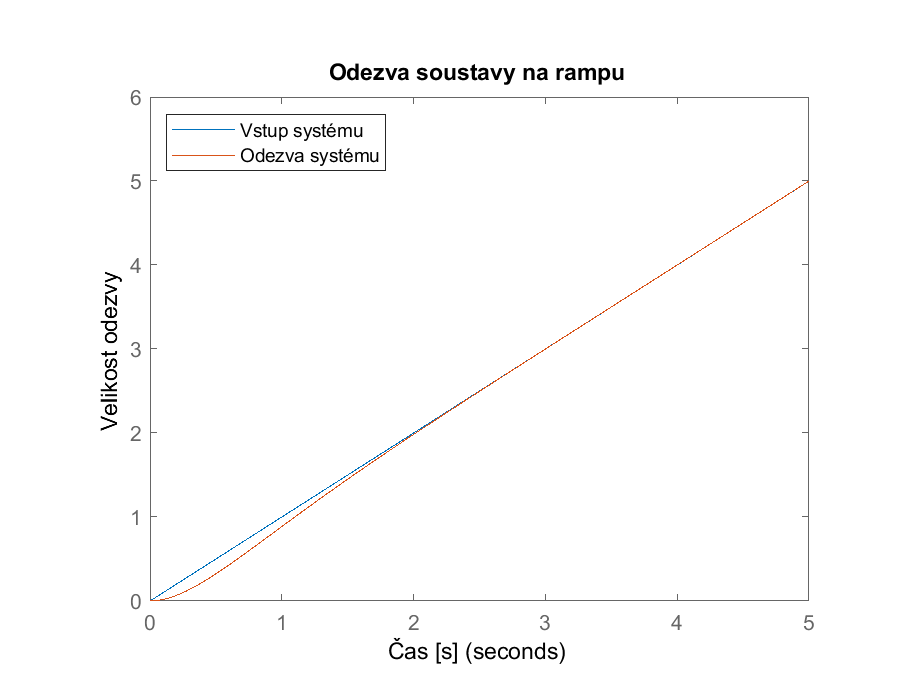
\includegraphics[width=.6\linewidth]{ramp_response.eps}
	\caption{Odezva soustavy na rampu}
	\label{fig:rampa}
\end{figure}
\begin{figure}[htbp]
	\centering
	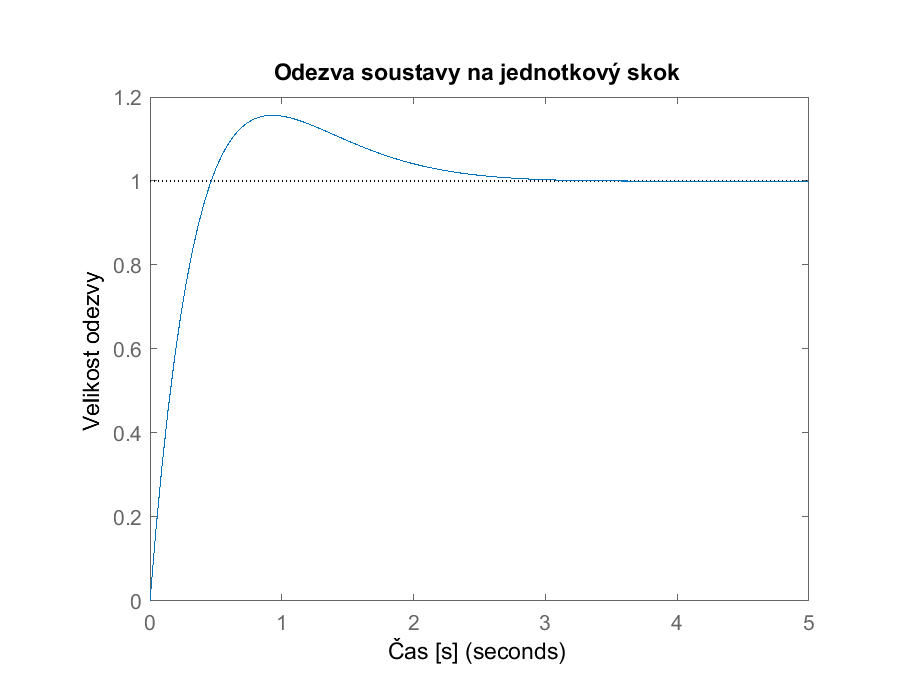
\includegraphics[width=.6\linewidth]{step_response.eps}
	\caption{Odezva soustavy na jednotkový skok}
	\label{fig:step}
\end{figure}

Na obrázku \ref{fig:rampa} je vykreslena odezva soustavy společně s rampou připojenou na vstup.
Na počátku je patrný přechodový děj, ale po několika vteřinách se soustava ustálí a rampu asymptoticky sleduje.

\begin{thebibliography}{9}


	\bibitem{sebek}
		prof. M. Šebek, přednášky ARI, FEL ČVUT, \url{http://www.polyx.com/_ari/slajdy/Bas-ARI-19-Polynom.pdf}
	
	\bibitem{motivace}
		Motivační hudba, \emph{Kirby dream land theme song} \url{https://www.youtube.com/watch?v=3CS93CdMv_E}
	
	\end{thebibliography}

\end{document}

